\section{Implementing Attacks}
\label{sec:implementattacks}

As we discovered during the software analysis, the Safeplug has a remote procedure call (RPC) capability.  This is a script called \verb!xspctrl! found in \verb!/opt/xce/html/svc! and it contains various options.  Particularly, functional calls to this script include enable and disable for all of the Safeplug settings, including Tor, ad block, and Tor relay.  None of them require any arguments in the POST string.

\begin{figure}[htb]
\begin{center}
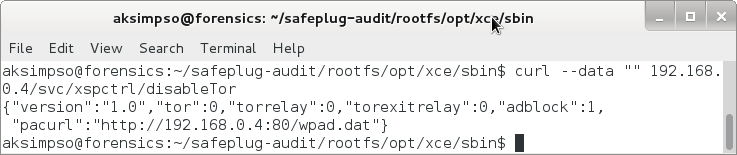
\includegraphics[width=.75\textwidth]{disabletor}
\caption{Disabling Tor as an insider attack.}
\label{disable}
\end{center}
\end{figure}

\subsection{Insider Attack}
Since the RPC server does not perform any kind of validation or authentication on the settings strings, it would be easy for anyone inside the local network to send a command and change the settings, for example to disable Tor or adblocking.  All the attacker would need to know is the IP of the device.  It does not even require SSH or discovering the (publically available) root password, or the user's new root password if they have been well-informed and adept enough to change it.  Figure \ref{disable} shows an example of this attack.

This attacker could also be any kind of device on the local network, or the local gateway if it is compromised.  The NSA ``Spymall'' catalog leaked in December shows tools for compromising a number of different devices and home routers are traditionally insecure \cite{spymall}.  It is easy to imagine any malicious party, not just one with the resources of a government, (although governments might be some of the most interested parties in attacking a Tor proxy) compromising the gateway and using that access make a disabling RPC call into the Safeplug.  This would occur silently from the perspective of a client unless the happen to check the Settings page for the Safeplug.  Instead, the client would continue browsing with a belief that they are protected by their use of the Tor network, while in fact any external adversary can track their traffic.

This seems like a fairly important vulnerability and requires action from Pogoplug to fix.  Since the purpose of these RPC operations is unclear without access to more of the source code, it is possible that they could be disabled entirely.  If not, perhaps there is some authentication protocol that could be implemented.  The challenge of such a protocol from a user's point of view is that valid access would be infrequent so giving a user a password to remember would be a poor experience.

\subsection{CSRF Attack}
An external website can also perform this attack by returning a correctly formatted POST string.  This executes the same functionality as the Insider Attack, but the attacker does not need to be on the local network or know the IP address of the Safeplug.  Instead, the attacker (who could be any malicious actor with access to a web server) can just send a POST request to every IP in the common ranges of local addresses in home networks, 192.168.0.0/24 and 192.168.1.0/24.  We implemented this attack with less than 30 lines of Javascript code (See Appendix A).  The following steps are necessary for the attack to be successful:

\begin{enumerate}
\item Set up a web page with the crafted Javascript code, which will send a POST request of the following format to all addresses in the range: \url{http://<IP address>/svc/xspctrl/disableTor} (See Appendix \ref{App:AppendixA}).
\item Send the malicious link to a user in the targeted private network.
\item Once the user clicks the link and loads the malicious site, the correctly formatted POST request will be sent to every IP address in the ranges.  
\item Tor is disabled silently.  The user must check or refresh her settings page to learn that Tor is turned off.  
\end{enumerate}  

This exploits the RPC server in the same manner that the Insider Attack does.  While this attack requires a greater amount of time because the local IP address of the Safeplug must be guessed via search, but the number of private address spaces is small, and the space likely to be occupied by a Safeplug on a home network is even smaller.  

The largest observed time to send requests to the 192.168.0.0/24 space was ~400 milliseconds; the entire attack costs ~800 milliseconds for sending request to both 192.168.0.0/24 and 192.168.1.0/24 ranges - even when the website was being loaded over Tor.  In the case of a private network in the range of 172.16.0.0/16, the attack took less than ~12 minutes (this generates script timeout warnings in most major browsers, which affects the timing of this attack).  This means that it would take a few hours to send requests to the full 172.16.0.0/12 range, which is commonly used in business networks.  The final private network space is 10.0.0.0/8 which is too large for an exhaustive search, but some simple optimization might make it feasible as well.  For example, using a GET request to get and parse the Safeplug settings page would allow the script to positively identify the safeplug and stop the search.  However, the 192.168.0.0/24 and 192.168.1.0/24 ranges are much more common in home networks; because Safeplug is geared towards home network use, in most cases the script will take less than a second, a trivial amount of time for the attacker to spend.  

In addition to disabling Tor, the attacker can modify any other settings on the device.  This includes: enabling/disabling Tor, enabling/disabling ad-blocking, enabling/disabling the use of the device as a Tor relay node [note: this requires the user to do additional setup], enabling/disabling the use of the device as an exit node (if it is already a relay).  Lastly, the attacker can also modify the user's whitelist of sites that should not be routed through Tor.  This whitelist attack is particularly dangerous because the change is silent and much harder for the user to notice the addition of a single website to the whitelist than a global loss of Tor.  (Removal of a webpage from the whitelist is likely to to cause usability problems and be more evident.)

\subsection{Gaining Access through SSH}
\label{sec:SSH}
    \subsubsection{Accessing the Device}
    Safeplug runs an RPC server that allows the enabling of SSH access via HTTP. SSH instructions for Cloud Engine's other device (Pogoplug) are widely available online and an email in the Tor-talk mailing list confirms that the instructions are the same (although the Pogoplug support staff note that SSH access breaks the warranty!) \cite{ceadmin}:
\begin{fileName}
curl --data ``'' http://<IP-of-Safeplug>/svc/xspctrl/enableSSHD
ssh root@<IP-of-Safeplug>
password: ceadmin
\end{fileName}

Obviously having a publically available root password means that SSH can be done effectively without authentication.  We tried the SSH procedure twice, once before the internet connection and activation, and once afterwards.  Before the activation and update procedure, SSH was not available.  The simple \verb!Hbplug! software on the box could not accept this RPC call.  However, once the box was updated and had lighttpd installed, the SSH procedure was available and we could download the contents of the root filesystem for analysis.
